\subsection{Resultados}
\par Llegados a el \'ultimo punto de este trabajo, ya se encuentran implementadas
    y experimentadas todas las heur\'isticas (y algorimto exacto) pedidas.

\par Ahora deseamos compara las heur\'isticas entre s\'i y llegar a nuevas
    conclusiones que no pudieron ser eval\'uadas al experimentar con cada
    una de ellas por separado.

\par De las mucha familias que se han presentado, hay muchas que tiene intersecciones
    nos vac\'ias (es decir, instancias en com\'un) y otras tantas que directamente
    son subfamilas de otras.

\par As\'i pues, sin necesidad de dar demasiados detalles al respecto, se
    puede afirmar que las \emph{Estrellas}, \emph{Banana Trees},
    \emph{Estrella+Puente+Doble Estrella} son subfamilias de los \emph{\'Arboles}.

\par A su vez, las estructuras internas de las familias \emph{Rueda}, \emph{Circular},
    son muy similiares a la de las \emph{Estrellas}, al menos para el contexto
    de las experimentaciones que fueron hechas y del problema sobre el que se est\'a
    trabajando. A su vez, estas 2 familias son de cierta ``estructura simple'' para
    la resoluci\'on de nuestro problema (al punto que el algoritmo exacto va a ser
    muy eficiente para instancias grandes de estos, a pesar de ser exponencial).

\par Por \'ultimo, y teniendo en cuenta lo que se dijo en \emph{\nameref{notas_preliminares}},
    como estamos trabajando sobre grafos conexos todos los grafos est\'an
    contenidos en las familias de grafos por densidad.

\par As\'i pues, con este panorama, decidimos elegir ciertas variantes de las
    heur\'isticas implementadas y realizar una experimentaci\'on de estas sobre
    los mismos conjuntos de instancias de ciertas familias. Como el problema
    no est\'a planteado para alg\'un tipo de grafo en com\'un, no se sabe
    si se desea obtener resultados particulares sobre ciertas familias, con
    lo cual decidimos utilizar para esta experimentaci\'on global a las familias
    de grafos por densidad (que incluyen a todas las dem\'as familias, sin limitarnos
    a ninguna estructura otra que ser conexas) y los \emph{\'Arboles}, estos \'ultimos
    por contener familias para los cuales se estuvo experimentando y a partir de
    cuyos resultados se eligen las variantes de las heur\'isticas que usaremos
    a continuaci\'on.

\par Sobre las variantes elegidas para esta experimentaci\'on, contamos con:

\begin{itemize}
    \item \textbf{El Algoritmo Exacto} Dicho algoritmo nos permitir\'a
        verificar cuan buenas son las soluciones dadas por las heur\'isticas,
        al menos para instancias chicas (pero que no son nada f\'aciles de
        resolver \emph{a mano}). Desde ya que est\'a descontado tratar
        de compara los tiempos de ejecuci\'on de las heur\'isticas con este
        algoritmo, requiriendo este evidentemente y sin demasiada necesidad de
        justificaci\'on, mucho m\'as tiempo para resolver los problemas.

    \item \textbf{Algoritmo Goloso} Siendo esta una heur\'istica para la
        cual no se plantearon variantes, pero habi\'endose usado como
        entrada de las otras dos, nos pareci\'o razonable utilizarla para
        verificar si las variantes que la utilizan como clique incial
        la mejoran o no.

    \item \textbf{B\'usqueda Local del mejor vecino con intercambio}, por
        lo explayado en la secci\'on de experimentaci\'on de esta
        heur\'istica, y sin tener ning\'un par\'ametro externo a utilizar
        para determinar cuando una heur\'istica es mejor que la otra (no
        sabemos el tiempo que se est\'a dispuesto a esperar por una respuesta
        ni cuan precisa debe ser esta), seleccionamos esta variante
        por ser una de las mejores para el \emph{tandem} tiempos de ejecuci\'on-%
        resultado devuelto.

    \item \textbf{B\'usqueda Tab\'u, \emph{MAX\_ITER = n, SIN\_MEJORAR = n,
        TIEMPO\_TABU = n/2}}, esta heur\'istica no recib\'e una entrada
        de la heur\'istica golosa y utiliza una funci\'on de aspiraci\'on.
        La seleccionamos por los mismos motivos que seleccionamos a la
        variante de b\'usqueda local.

    \item \textbf{B\'usqueda Tab\'u, \emph{MAX\_ITER = n, SIN\_MEJORAR = n,
        TIEMPO\_TABU = n/2}}, esta heur\'istica si recib\'e una entrada
        por parte de la heur\'istica golosa y no utiliza una funci\'on
        de aspiraci\'on. Fue seleccionada por los mismos motivoos
        que la otra variante de b\'usqueda tab\'u.
\end{itemize}

\subsubsection{\'Arboles}
%Tree
\begin{figure}[H]
    \centering
    \fontsize{7}{10}\selectfont
    \resizebox{0.80\textwidth}{!}{% GNUPLOT: LaTeX picture with Postscript
\begingroup
  \makeatletter
  \providecommand\color[2][]{%
    \GenericError{(gnuplot) \space\space\space\@spaces}{%
      Package color not loaded in conjunction with
      terminal option `colourtext'%
    }{See the gnuplot documentation for explanation.%
    }{Either use 'blacktext' in gnuplot or load the package
      color.sty in LaTeX.}%
    \renewcommand\color[2][]{}%
  }%
  \providecommand\includegraphics[2][]{%
    \GenericError{(gnuplot) \space\space\space\@spaces}{%
      Package graphicx or graphics not loaded%
    }{See the gnuplot documentation for explanation.%
    }{The gnuplot epslatex terminal needs graphicx.sty or graphics.sty.}%
    \renewcommand\includegraphics[2][]{}%
  }%
  \providecommand\rotatebox[2]{#2}%
  \@ifundefined{ifGPcolor}{%
    \newif\ifGPcolor
    \GPcolortrue
  }{}%
  \@ifundefined{ifGPblacktext}{%
    \newif\ifGPblacktext
    \GPblacktexttrue
  }{}%
  % define a \g@addto@macro without @ in the name:
  \let\gplgaddtomacro\g@addto@macro
  % define empty templates for all commands taking text:
  \gdef\gplbacktext{}%
  \gdef\gplfronttext{}%
  \makeatother
  \ifGPblacktext
    % no textcolor at all
    \def\colorrgb#1{}%
    \def\colorgray#1{}%
  \else
    % gray or color?
    \ifGPcolor
      \def\colorrgb#1{\color[rgb]{#1}}%
      \def\colorgray#1{\color[gray]{#1}}%
      \expandafter\def\csname LTw\endcsname{\color{white}}%
      \expandafter\def\csname LTb\endcsname{\color{black}}%
      \expandafter\def\csname LTa\endcsname{\color{black}}%
      \expandafter\def\csname LT0\endcsname{\color[rgb]{1,0,0}}%
      \expandafter\def\csname LT1\endcsname{\color[rgb]{0,1,0}}%
      \expandafter\def\csname LT2\endcsname{\color[rgb]{0,0,1}}%
      \expandafter\def\csname LT3\endcsname{\color[rgb]{1,0,1}}%
      \expandafter\def\csname LT4\endcsname{\color[rgb]{0,1,1}}%
      \expandafter\def\csname LT5\endcsname{\color[rgb]{1,1,0}}%
      \expandafter\def\csname LT6\endcsname{\color[rgb]{0,0,0}}%
      \expandafter\def\csname LT7\endcsname{\color[rgb]{1,0.3,0}}%
      \expandafter\def\csname LT8\endcsname{\color[rgb]{0.5,0.5,0.5}}%
    \else
      % gray
      \def\colorrgb#1{\color{black}}%
      \def\colorgray#1{\color[gray]{#1}}%
      \expandafter\def\csname LTw\endcsname{\color{white}}%
      \expandafter\def\csname LTb\endcsname{\color{black}}%
      \expandafter\def\csname LTa\endcsname{\color{black}}%
      \expandafter\def\csname LT0\endcsname{\color{black}}%
      \expandafter\def\csname LT1\endcsname{\color{black}}%
      \expandafter\def\csname LT2\endcsname{\color{black}}%
      \expandafter\def\csname LT3\endcsname{\color{black}}%
      \expandafter\def\csname LT4\endcsname{\color{black}}%
      \expandafter\def\csname LT5\endcsname{\color{black}}%
      \expandafter\def\csname LT6\endcsname{\color{black}}%
      \expandafter\def\csname LT7\endcsname{\color{black}}%
      \expandafter\def\csname LT8\endcsname{\color{black}}%
    \fi
  \fi
  \setlength{\unitlength}{0.0500bp}%
  \begin{picture}(7200.00,5040.00)%
    \gplgaddtomacro\gplbacktext{%
      \csname LTb\endcsname%
      \put(1562,2244){\makebox(0,0)[r]{\strut{} 0.1}}%
      \csname LTb\endcsname%
      \put(1562,2600){\makebox(0,0)[r]{\strut{} 1}}%
      \csname LTb\endcsname%
      \put(1562,2956){\makebox(0,0)[r]{\strut{} 10}}%
      \csname LTb\endcsname%
      \put(1562,3312){\makebox(0,0)[r]{\strut{} 100}}%
      \csname LTb\endcsname%
      \put(1562,3667){\makebox(0,0)[r]{\strut{} 1000}}%
      \csname LTb\endcsname%
      \put(1562,4023){\makebox(0,0)[r]{\strut{} 10000}}%
      \csname LTb\endcsname%
      \put(1562,4379){\makebox(0,0)[r]{\strut{} 100000}}%
      \csname LTb\endcsname%
      \put(1694,2024){\makebox(0,0){\strut{} 0}}%
      \csname LTb\endcsname%
      \put(2205,2024){\makebox(0,0){\strut{} 500}}%
      \csname LTb\endcsname%
      \put(2716,2024){\makebox(0,0){\strut{} 1000}}%
      \csname LTb\endcsname%
      \put(3227,2024){\makebox(0,0){\strut{} 1500}}%
      \csname LTb\endcsname%
      \put(3738,2024){\makebox(0,0){\strut{} 2000}}%
      \csname LTb\endcsname%
      \put(4249,2024){\makebox(0,0){\strut{} 2500}}%
      \csname LTb\endcsname%
      \put(4759,2024){\makebox(0,0){\strut{} 3000}}%
      \csname LTb\endcsname%
      \put(5270,2024){\makebox(0,0){\strut{} 3500}}%
      \csname LTb\endcsname%
      \put(5781,2024){\makebox(0,0){\strut{} 4000}}%
      \csname LTb\endcsname%
      \put(6292,2024){\makebox(0,0){\strut{} 4500}}%
      \csname LTb\endcsname%
      \put(6803,2024){\makebox(0,0){\strut{} 5000}}%
      \put(176,3311){\rotatebox{-270}{\makebox(0,0){\strut{}Tiempo (microsegundos)}}}%
      \put(396,3311){\rotatebox{-270}{\makebox(0,0){\strut{}(Escala Logaritmica)}}}%
      \put(4248,1694){\makebox(0,0){\strut{}Cantidad de Nodos}}%
      \put(4248,1474){\makebox(0,0){\strut{}(Escala Lineal)}}%
      \put(4248,4709){\makebox(0,0){\strut{}Tiempo de ejecucion conforme aumenta la cantidad de nodos}}%
    }%
    \gplgaddtomacro\gplfronttext{%
      \csname LTb\endcsname%
      \put(6263,1053){\makebox(0,0)[r]{\strut{}Algoritmo Exacto}}%
      \csname LTb\endcsname%
      \put(6263,833){\makebox(0,0)[r]{\strut{}Tabu(n,n,n/2) (golosa,sin aspiracion)}}%
      \csname LTb\endcsname%
      \put(6263,613){\makebox(0,0)[r]{\strut{}Tabu(n,n,n/2)}}%
      \csname LTb\endcsname%
      \put(6263,393){\makebox(0,0)[r]{\strut{}BL (mejor vecino,intercambio)}}%
      \csname LTb\endcsname%
      \put(6263,173){\makebox(0,0)[r]{\strut{}Golosa}}%
    }%
    \gplbacktext
    \put(0,0){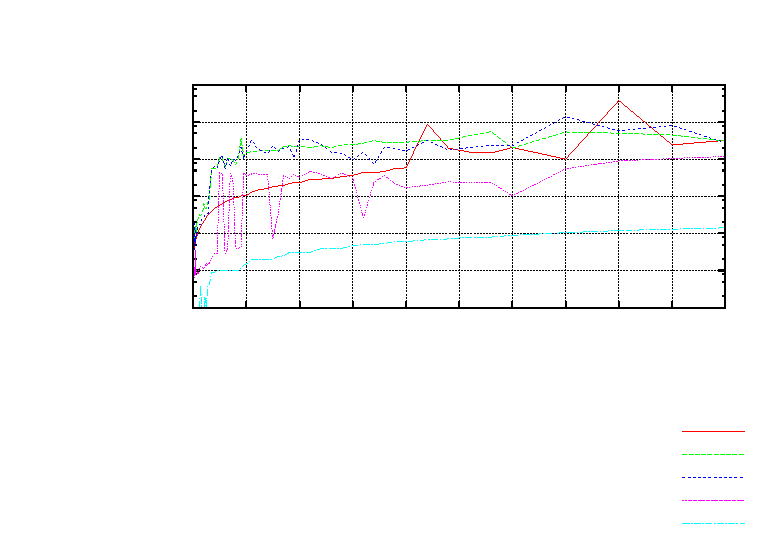
\includegraphics{ej4_nodos_tree}}%
    \gplfronttext
  \end{picture}%
\endgroup
}
    \caption{Complejidad temporal para \'Arboles}
\end{figure}

\begin{figure}[H]
    \centering
    \fontsize{7}{10}\selectfont
    \resizebox{0.80\textwidth}{!}{% GNUPLOT: LaTeX picture with Postscript
\begingroup
  \makeatletter
  \providecommand\color[2][]{%
    \GenericError{(gnuplot) \space\space\space\@spaces}{%
      Package color not loaded in conjunction with
      terminal option `colourtext'%
    }{See the gnuplot documentation for explanation.%
    }{Either use 'blacktext' in gnuplot or load the package
      color.sty in LaTeX.}%
    \renewcommand\color[2][]{}%
  }%
  \providecommand\includegraphics[2][]{%
    \GenericError{(gnuplot) \space\space\space\@spaces}{%
      Package graphicx or graphics not loaded%
    }{See the gnuplot documentation for explanation.%
    }{The gnuplot epslatex terminal needs graphicx.sty or graphics.sty.}%
    \renewcommand\includegraphics[2][]{}%
  }%
  \providecommand\rotatebox[2]{#2}%
  \@ifundefined{ifGPcolor}{%
    \newif\ifGPcolor
    \GPcolortrue
  }{}%
  \@ifundefined{ifGPblacktext}{%
    \newif\ifGPblacktext
    \GPblacktexttrue
  }{}%
  % define a \g@addto@macro without @ in the name:
  \let\gplgaddtomacro\g@addto@macro
  % define empty templates for all commands taking text:
  \gdef\gplbacktext{}%
  \gdef\gplfronttext{}%
  \makeatother
  \ifGPblacktext
    % no textcolor at all
    \def\colorrgb#1{}%
    \def\colorgray#1{}%
  \else
    % gray or color?
    \ifGPcolor
      \def\colorrgb#1{\color[rgb]{#1}}%
      \def\colorgray#1{\color[gray]{#1}}%
      \expandafter\def\csname LTw\endcsname{\color{white}}%
      \expandafter\def\csname LTb\endcsname{\color{black}}%
      \expandafter\def\csname LTa\endcsname{\color{black}}%
      \expandafter\def\csname LT0\endcsname{\color[rgb]{1,0,0}}%
      \expandafter\def\csname LT1\endcsname{\color[rgb]{0,1,0}}%
      \expandafter\def\csname LT2\endcsname{\color[rgb]{0,0,1}}%
      \expandafter\def\csname LT3\endcsname{\color[rgb]{1,0,1}}%
      \expandafter\def\csname LT4\endcsname{\color[rgb]{0,1,1}}%
      \expandafter\def\csname LT5\endcsname{\color[rgb]{1,1,0}}%
      \expandafter\def\csname LT6\endcsname{\color[rgb]{0,0,0}}%
      \expandafter\def\csname LT7\endcsname{\color[rgb]{1,0.3,0}}%
      \expandafter\def\csname LT8\endcsname{\color[rgb]{0.5,0.5,0.5}}%
    \else
      % gray
      \def\colorrgb#1{\color{black}}%
      \def\colorgray#1{\color[gray]{#1}}%
      \expandafter\def\csname LTw\endcsname{\color{white}}%
      \expandafter\def\csname LTb\endcsname{\color{black}}%
      \expandafter\def\csname LTa\endcsname{\color{black}}%
      \expandafter\def\csname LT0\endcsname{\color{black}}%
      \expandafter\def\csname LT1\endcsname{\color{black}}%
      \expandafter\def\csname LT2\endcsname{\color{black}}%
      \expandafter\def\csname LT3\endcsname{\color{black}}%
      \expandafter\def\csname LT4\endcsname{\color{black}}%
      \expandafter\def\csname LT5\endcsname{\color{black}}%
      \expandafter\def\csname LT6\endcsname{\color{black}}%
      \expandafter\def\csname LT7\endcsname{\color{black}}%
      \expandafter\def\csname LT8\endcsname{\color{black}}%
    \fi
  \fi
  \setlength{\unitlength}{0.0500bp}%
  \begin{picture}(7200.00,5040.00)%
    \gplgaddtomacro\gplbacktext{%
      \csname LTb\endcsname%
      \put(1034,2244){\makebox(0,0)[r]{\strut{} 0}}%
      \csname LTb\endcsname%
      \put(1034,2671){\makebox(0,0)[r]{\strut{} 5}}%
      \csname LTb\endcsname%
      \put(1034,3098){\makebox(0,0)[r]{\strut{} 10}}%
      \csname LTb\endcsname%
      \put(1034,3525){\makebox(0,0)[r]{\strut{} 15}}%
      \csname LTb\endcsname%
      \put(1034,3952){\makebox(0,0)[r]{\strut{} 20}}%
      \csname LTb\endcsname%
      \put(1034,4379){\makebox(0,0)[r]{\strut{} 25}}%
      \csname LTb\endcsname%
      \put(1166,2024){\makebox(0,0){\strut{} 1}}%
      \csname LTb\endcsname%
      \put(2575,2024){\makebox(0,0){\strut{} 10}}%
      \csname LTb\endcsname%
      \put(3985,2024){\makebox(0,0){\strut{} 100}}%
      \csname LTb\endcsname%
      \put(5394,2024){\makebox(0,0){\strut{} 1000}}%
      \csname LTb\endcsname%
      \put(6803,2024){\makebox(0,0){\strut{} 10000}}%
      \put(176,3311){\rotatebox{-270}{\makebox(0,0){\strut{}Frontera}}}%
      \put(396,3311){\rotatebox{-270}{\makebox(0,0){\strut{}(Escala Lineal)}}}%
      \put(3984,1694){\makebox(0,0){\strut{}Cantidad de Nodos}}%
      \put(3984,1474){\makebox(0,0){\strut{}(Escala Logaritmica)}}%
      \put(3984,4709){\makebox(0,0){\strut{}Frontera obtenida segun cantidad de nodos}}%
    }%
    \gplgaddtomacro\gplfronttext{%
      \csname LTb\endcsname%
      \put(5999,1053){\makebox(0,0)[r]{\strut{}Algoritmo Exacto}}%
      \csname LTb\endcsname%
      \put(5999,833){\makebox(0,0)[r]{\strut{}Tabu(n,n,n/2) (golosa,sin aspiracion)}}%
      \csname LTb\endcsname%
      \put(5999,613){\makebox(0,0)[r]{\strut{}Tabu(n,n,n/2)}}%
      \csname LTb\endcsname%
      \put(5999,393){\makebox(0,0)[r]{\strut{}BL (mejor vecino,intercambio)}}%
      \csname LTb\endcsname%
      \put(5999,173){\makebox(0,0)[r]{\strut{}Golosa}}%
    }%
    \gplbacktext
    \put(0,0){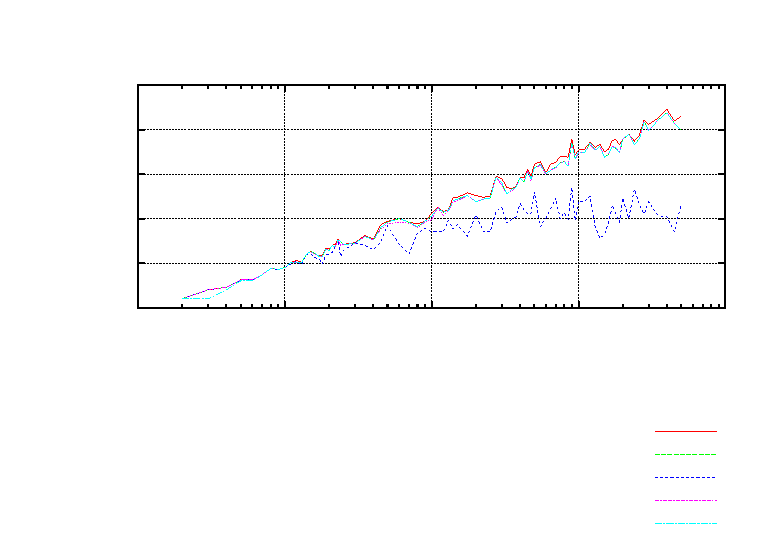
\includegraphics{ej4_frontera_tree}}%
    \gplfronttext
  \end{picture}%
\endgroup
}
    \caption{Frontera para \'Arboles}
\end{figure}

\bigskip

\par Para la familia de los grafos el primer resultado evidente que podemos
    indicar es que la golosa es la mejor opci\'on sin lugar a dudas.

\par Mientras que el resto de las heur\'isticas an\'alizadas oscila en un
    coste temporal de entre 100 a 100000 mil microsegundos de diferencia
    con la golosa (la cual se va incrementando a medida que se incrementa
    el tama\~no de la entrada), el resultado provisto por la golosa
    es id\'entico al ex\'acto o est\'a muy cerca de cerlo.

\par Sin lugar a dudas, en el caso de trabajar con \'arboles (y a pesar
    de la familia $Estrella+Puente+Doble Estrella$, que es un caso
    particular de la familia $Estrella+Puente+CMF$ (sobre la cual
    esta heur\'istica no funciona bien), est\'a heur\'istica
    tiene (para los datos que manejamos de requerimientos a la hora
    de resolver el problema) el mejor balance tiempo-resultado.

\subsubsection{Grafos poco densos}
%Connected Sparse
\begin{figure}[H]
    \centering
    \fontsize{7}{10}\selectfont
    \resizebox{0.80\textwidth}{!}{% GNUPLOT: LaTeX picture with Postscript
\begingroup
  \makeatletter
  \providecommand\color[2][]{%
    \GenericError{(gnuplot) \space\space\space\@spaces}{%
      Package color not loaded in conjunction with
      terminal option `colourtext'%
    }{See the gnuplot documentation for explanation.%
    }{Either use 'blacktext' in gnuplot or load the package
      color.sty in LaTeX.}%
    \renewcommand\color[2][]{}%
  }%
  \providecommand\includegraphics[2][]{%
    \GenericError{(gnuplot) \space\space\space\@spaces}{%
      Package graphicx or graphics not loaded%
    }{See the gnuplot documentation for explanation.%
    }{The gnuplot epslatex terminal needs graphicx.sty or graphics.sty.}%
    \renewcommand\includegraphics[2][]{}%
  }%
  \providecommand\rotatebox[2]{#2}%
  \@ifundefined{ifGPcolor}{%
    \newif\ifGPcolor
    \GPcolortrue
  }{}%
  \@ifundefined{ifGPblacktext}{%
    \newif\ifGPblacktext
    \GPblacktexttrue
  }{}%
  % define a \g@addto@macro without @ in the name:
  \let\gplgaddtomacro\g@addto@macro
  % define empty templates for all commands taking text:
  \gdef\gplbacktext{}%
  \gdef\gplfronttext{}%
  \makeatother
  \ifGPblacktext
    % no textcolor at all
    \def\colorrgb#1{}%
    \def\colorgray#1{}%
  \else
    % gray or color?
    \ifGPcolor
      \def\colorrgb#1{\color[rgb]{#1}}%
      \def\colorgray#1{\color[gray]{#1}}%
      \expandafter\def\csname LTw\endcsname{\color{white}}%
      \expandafter\def\csname LTb\endcsname{\color{black}}%
      \expandafter\def\csname LTa\endcsname{\color{black}}%
      \expandafter\def\csname LT0\endcsname{\color[rgb]{1,0,0}}%
      \expandafter\def\csname LT1\endcsname{\color[rgb]{0,1,0}}%
      \expandafter\def\csname LT2\endcsname{\color[rgb]{0,0,1}}%
      \expandafter\def\csname LT3\endcsname{\color[rgb]{1,0,1}}%
      \expandafter\def\csname LT4\endcsname{\color[rgb]{0,1,1}}%
      \expandafter\def\csname LT5\endcsname{\color[rgb]{1,1,0}}%
      \expandafter\def\csname LT6\endcsname{\color[rgb]{0,0,0}}%
      \expandafter\def\csname LT7\endcsname{\color[rgb]{1,0.3,0}}%
      \expandafter\def\csname LT8\endcsname{\color[rgb]{0.5,0.5,0.5}}%
    \else
      % gray
      \def\colorrgb#1{\color{black}}%
      \def\colorgray#1{\color[gray]{#1}}%
      \expandafter\def\csname LTw\endcsname{\color{white}}%
      \expandafter\def\csname LTb\endcsname{\color{black}}%
      \expandafter\def\csname LTa\endcsname{\color{black}}%
      \expandafter\def\csname LT0\endcsname{\color{black}}%
      \expandafter\def\csname LT1\endcsname{\color{black}}%
      \expandafter\def\csname LT2\endcsname{\color{black}}%
      \expandafter\def\csname LT3\endcsname{\color{black}}%
      \expandafter\def\csname LT4\endcsname{\color{black}}%
      \expandafter\def\csname LT5\endcsname{\color{black}}%
      \expandafter\def\csname LT6\endcsname{\color{black}}%
      \expandafter\def\csname LT7\endcsname{\color{black}}%
      \expandafter\def\csname LT8\endcsname{\color{black}}%
    \fi
  \fi
  \setlength{\unitlength}{0.0500bp}%
  \begin{picture}(7200.00,5040.00)%
    \gplgaddtomacro\gplbacktext{%
      \csname LTb\endcsname%
      \put(1562,2244){\makebox(0,0)[r]{\strut{} 0.1}}%
      \csname LTb\endcsname%
      \put(1562,2458){\makebox(0,0)[r]{\strut{} 1}}%
      \csname LTb\endcsname%
      \put(1562,2671){\makebox(0,0)[r]{\strut{} 10}}%
      \csname LTb\endcsname%
      \put(1562,2885){\makebox(0,0)[r]{\strut{} 100}}%
      \csname LTb\endcsname%
      \put(1562,3098){\makebox(0,0)[r]{\strut{} 1000}}%
      \csname LTb\endcsname%
      \put(1562,3312){\makebox(0,0)[r]{\strut{} 10000}}%
      \csname LTb\endcsname%
      \put(1562,3525){\makebox(0,0)[r]{\strut{} 100000}}%
      \csname LTb\endcsname%
      \put(1562,3739){\makebox(0,0)[r]{\strut{} 1e+06}}%
      \csname LTb\endcsname%
      \put(1562,3952){\makebox(0,0)[r]{\strut{} 1e+07}}%
      \csname LTb\endcsname%
      \put(1562,4166){\makebox(0,0)[r]{\strut{} 1e+08}}%
      \csname LTb\endcsname%
      \put(1562,4379){\makebox(0,0)[r]{\strut{} 1e+09}}%
      \csname LTb\endcsname%
      \put(1694,2024){\makebox(0,0){\strut{} 0}}%
      \csname LTb\endcsname%
      \put(2205,2024){\makebox(0,0){\strut{} 500}}%
      \csname LTb\endcsname%
      \put(2716,2024){\makebox(0,0){\strut{} 1000}}%
      \csname LTb\endcsname%
      \put(3227,2024){\makebox(0,0){\strut{} 1500}}%
      \csname LTb\endcsname%
      \put(3738,2024){\makebox(0,0){\strut{} 2000}}%
      \csname LTb\endcsname%
      \put(4249,2024){\makebox(0,0){\strut{} 2500}}%
      \csname LTb\endcsname%
      \put(4759,2024){\makebox(0,0){\strut{} 3000}}%
      \csname LTb\endcsname%
      \put(5270,2024){\makebox(0,0){\strut{} 3500}}%
      \csname LTb\endcsname%
      \put(5781,2024){\makebox(0,0){\strut{} 4000}}%
      \csname LTb\endcsname%
      \put(6292,2024){\makebox(0,0){\strut{} 4500}}%
      \csname LTb\endcsname%
      \put(6803,2024){\makebox(0,0){\strut{} 5000}}%
      \put(176,3311){\rotatebox{-270}{\makebox(0,0){\strut{}Tiempo (microsegundos)}}}%
      \put(396,3311){\rotatebox{-270}{\makebox(0,0){\strut{}(Escala Logaritmica)}}}%
      \put(4248,1694){\makebox(0,0){\strut{}Cantidad de Nodos}}%
      \put(4248,1474){\makebox(0,0){\strut{}(Escala Lineal)}}%
      \put(4248,4709){\makebox(0,0){\strut{}Tiempo de ejecucion conforme aumenta la cantidad de nodos}}%
    }%
    \gplgaddtomacro\gplfronttext{%
      \csname LTb\endcsname%
      \put(6131,1053){\makebox(0,0)[r]{\strut{}Algoritmo Exacto}}%
      \csname LTb\endcsname%
      \put(6131,833){\makebox(0,0)[r]{\strut{}Tabu(n,n,n/2,golosa,sin aspiracion)}}%
      \csname LTb\endcsname%
      \put(6131,613){\makebox(0,0)[r]{\strut{}Tabu(n,n,n/2)}}%
      \csname LTb\endcsname%
      \put(6131,393){\makebox(0,0)[r]{\strut{}BL(mejor vecino,intercambio)}}%
      \csname LTb\endcsname%
      \put(6131,173){\makebox(0,0)[r]{\strut{}Golosa}}%
    }%
    \gplbacktext
    \put(0,0){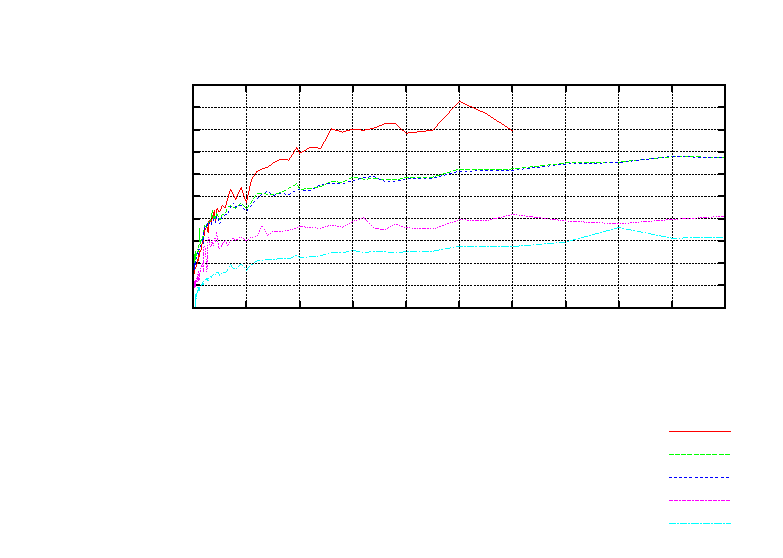
\includegraphics{ej4_nodos_connected_sparse}}%
    \gplfronttext
  \end{picture}%
\endgroup
}
    \caption{Complejidad temporal para Grafos Conexos Poco Densos}
\end{figure}

\begin{figure}[H]
    \centering
    \fontsize{7}{10}\selectfont
    \resizebox{0.80\textwidth}{!}{% GNUPLOT: LaTeX picture with Postscript
\begingroup
  \makeatletter
  \providecommand\color[2][]{%
    \GenericError{(gnuplot) \space\space\space\@spaces}{%
      Package color not loaded in conjunction with
      terminal option `colourtext'%
    }{See the gnuplot documentation for explanation.%
    }{Either use 'blacktext' in gnuplot or load the package
      color.sty in LaTeX.}%
    \renewcommand\color[2][]{}%
  }%
  \providecommand\includegraphics[2][]{%
    \GenericError{(gnuplot) \space\space\space\@spaces}{%
      Package graphicx or graphics not loaded%
    }{See the gnuplot documentation for explanation.%
    }{The gnuplot epslatex terminal needs graphicx.sty or graphics.sty.}%
    \renewcommand\includegraphics[2][]{}%
  }%
  \providecommand\rotatebox[2]{#2}%
  \@ifundefined{ifGPcolor}{%
    \newif\ifGPcolor
    \GPcolortrue
  }{}%
  \@ifundefined{ifGPblacktext}{%
    \newif\ifGPblacktext
    \GPblacktexttrue
  }{}%
  % define a \g@addto@macro without @ in the name:
  \let\gplgaddtomacro\g@addto@macro
  % define empty templates for all commands taking text:
  \gdef\gplbacktext{}%
  \gdef\gplfronttext{}%
  \makeatother
  \ifGPblacktext
    % no textcolor at all
    \def\colorrgb#1{}%
    \def\colorgray#1{}%
  \else
    % gray or color?
    \ifGPcolor
      \def\colorrgb#1{\color[rgb]{#1}}%
      \def\colorgray#1{\color[gray]{#1}}%
      \expandafter\def\csname LTw\endcsname{\color{white}}%
      \expandafter\def\csname LTb\endcsname{\color{black}}%
      \expandafter\def\csname LTa\endcsname{\color{black}}%
      \expandafter\def\csname LT0\endcsname{\color[rgb]{1,0,0}}%
      \expandafter\def\csname LT1\endcsname{\color[rgb]{0,1,0}}%
      \expandafter\def\csname LT2\endcsname{\color[rgb]{0,0,1}}%
      \expandafter\def\csname LT3\endcsname{\color[rgb]{1,0,1}}%
      \expandafter\def\csname LT4\endcsname{\color[rgb]{0,1,1}}%
      \expandafter\def\csname LT5\endcsname{\color[rgb]{1,1,0}}%
      \expandafter\def\csname LT6\endcsname{\color[rgb]{0,0,0}}%
      \expandafter\def\csname LT7\endcsname{\color[rgb]{1,0.3,0}}%
      \expandafter\def\csname LT8\endcsname{\color[rgb]{0.5,0.5,0.5}}%
    \else
      % gray
      \def\colorrgb#1{\color{black}}%
      \def\colorgray#1{\color[gray]{#1}}%
      \expandafter\def\csname LTw\endcsname{\color{white}}%
      \expandafter\def\csname LTb\endcsname{\color{black}}%
      \expandafter\def\csname LTa\endcsname{\color{black}}%
      \expandafter\def\csname LT0\endcsname{\color{black}}%
      \expandafter\def\csname LT1\endcsname{\color{black}}%
      \expandafter\def\csname LT2\endcsname{\color{black}}%
      \expandafter\def\csname LT3\endcsname{\color{black}}%
      \expandafter\def\csname LT4\endcsname{\color{black}}%
      \expandafter\def\csname LT5\endcsname{\color{black}}%
      \expandafter\def\csname LT6\endcsname{\color{black}}%
      \expandafter\def\csname LT7\endcsname{\color{black}}%
      \expandafter\def\csname LT8\endcsname{\color{black}}%
    \fi
  \fi
  \setlength{\unitlength}{0.0500bp}%
  \begin{picture}(7200.00,5040.00)%
    \gplgaddtomacro\gplbacktext{%
      \csname LTb\endcsname%
      \put(1298,2244){\makebox(0,0)[r]{\strut{} 0}}%
      \csname LTb\endcsname%
      \put(1298,2511){\makebox(0,0)[r]{\strut{} 1000}}%
      \csname LTb\endcsname%
      \put(1298,2778){\makebox(0,0)[r]{\strut{} 2000}}%
      \csname LTb\endcsname%
      \put(1298,3045){\makebox(0,0)[r]{\strut{} 3000}}%
      \csname LTb\endcsname%
      \put(1298,3312){\makebox(0,0)[r]{\strut{} 4000}}%
      \csname LTb\endcsname%
      \put(1298,3578){\makebox(0,0)[r]{\strut{} 5000}}%
      \csname LTb\endcsname%
      \put(1298,3845){\makebox(0,0)[r]{\strut{} 6000}}%
      \csname LTb\endcsname%
      \put(1298,4112){\makebox(0,0)[r]{\strut{} 7000}}%
      \csname LTb\endcsname%
      \put(1298,4379){\makebox(0,0)[r]{\strut{} 8000}}%
      \csname LTb\endcsname%
      \put(1430,2024){\makebox(0,0){\strut{} 0}}%
      \csname LTb\endcsname%
      \put(1967,2024){\makebox(0,0){\strut{} 500}}%
      \csname LTb\endcsname%
      \put(2505,2024){\makebox(0,0){\strut{} 1000}}%
      \csname LTb\endcsname%
      \put(3042,2024){\makebox(0,0){\strut{} 1500}}%
      \csname LTb\endcsname%
      \put(3579,2024){\makebox(0,0){\strut{} 2000}}%
      \csname LTb\endcsname%
      \put(4117,2024){\makebox(0,0){\strut{} 2500}}%
      \csname LTb\endcsname%
      \put(4654,2024){\makebox(0,0){\strut{} 3000}}%
      \csname LTb\endcsname%
      \put(5191,2024){\makebox(0,0){\strut{} 3500}}%
      \csname LTb\endcsname%
      \put(5728,2024){\makebox(0,0){\strut{} 4000}}%
      \csname LTb\endcsname%
      \put(6266,2024){\makebox(0,0){\strut{} 4500}}%
      \csname LTb\endcsname%
      \put(6803,2024){\makebox(0,0){\strut{} 5000}}%
      \put(176,3311){\rotatebox{-270}{\makebox(0,0){\strut{}Frontera}}}%
      \put(396,3311){\rotatebox{-270}{\makebox(0,0){\strut{}(Escala Lineal)}}}%
      \put(4116,1694){\makebox(0,0){\strut{}Cantidad de Nodos}}%
      \put(4116,1474){\makebox(0,0){\strut{}(Escala Lineal)}}%
      \put(4116,4709){\makebox(0,0){\strut{}Frontera obtenida segun cantidad de nodos}}%
    }%
    \gplgaddtomacro\gplfronttext{%
      \csname LTb\endcsname%
      \put(5999,1053){\makebox(0,0)[r]{\strut{}Algoritmo Exacto}}%
      \csname LTb\endcsname%
      \put(5999,833){\makebox(0,0)[r]{\strut{}Tabu(n,n,n/2,golosa,sin aspiracion)}}%
      \csname LTb\endcsname%
      \put(5999,613){\makebox(0,0)[r]{\strut{}Tabu(n,n,n/2)}}%
      \csname LTb\endcsname%
      \put(5999,393){\makebox(0,0)[r]{\strut{}BL(mejor vecino,intercambio)}}%
      \csname LTb\endcsname%
      \put(5999,173){\makebox(0,0)[r]{\strut{}Golosa}}%
    }%
    \gplbacktext
    \put(0,0){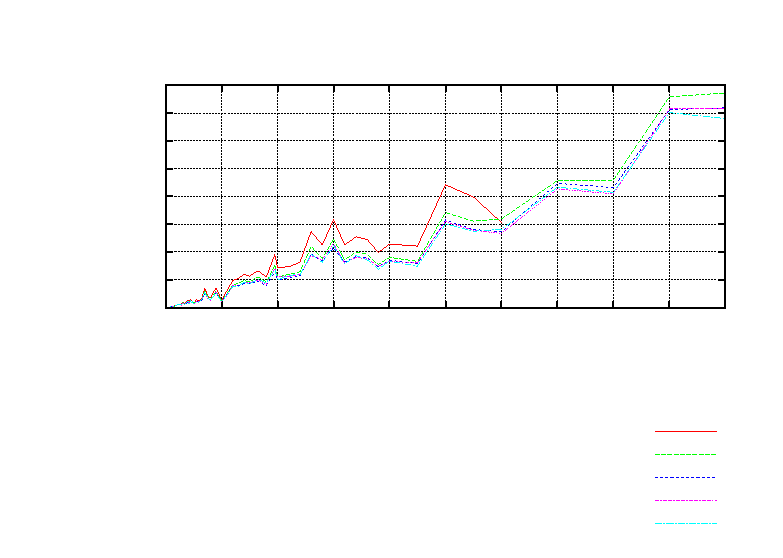
\includegraphics{ej4_frontera_connected_sparse}}%
    \gplfronttext
  \end{picture}%
\endgroup
}
    \caption{Frontera para Grafos Conexos Poco Densos}
\end{figure}

\bigskip

\par Al igual que con los \'arboles, se observa para este tipo
    de grafos un comportamiento similiar (sino id\'entico) en la
    familia de grafos poco densos.

\par Sin ir m\'as lejos, los \'arboles son grafos conexos poco densos
    (de hecho, son los grafos conexos menos densos que hay, ya que
    por ser \'arboles, si se le quita cualquier arista, deja de ser
    conexo).

\par Nuevamente se observa como la heur\'istica golosa requiere menos
    tiempo que todas las dem\'as para terminar (aunque est\'a seguida
    de cerca por la variante de la b\'usqueda local).

\par Y, en cuanto al resultado, vemos que no est\'a m\'as lejos de
    la soluci\'on del algoritmo exacto que las dem\'as heur\'isticas
    (en particular, para las instancias en las que se pudo correr
    el algoritmo exacto -por limitaciones de tiempo-, las heur\'isticas
    est\'an razonablemente cerca de la soluci\'on \'optima).

\subsubsection{Grafos regularmente densos}
%Connected Regular
\begin{figure}[H]
    \centering
    \fontsize{7}{10}\selectfont
    \resizebox{0.80\textwidth}{!}{% GNUPLOT: LaTeX picture with Postscript
\begingroup
  \makeatletter
  \providecommand\color[2][]{%
    \GenericError{(gnuplot) \space\space\space\@spaces}{%
      Package color not loaded in conjunction with
      terminal option `colourtext'%
    }{See the gnuplot documentation for explanation.%
    }{Either use 'blacktext' in gnuplot or load the package
      color.sty in LaTeX.}%
    \renewcommand\color[2][]{}%
  }%
  \providecommand\includegraphics[2][]{%
    \GenericError{(gnuplot) \space\space\space\@spaces}{%
      Package graphicx or graphics not loaded%
    }{See the gnuplot documentation for explanation.%
    }{The gnuplot epslatex terminal needs graphicx.sty or graphics.sty.}%
    \renewcommand\includegraphics[2][]{}%
  }%
  \providecommand\rotatebox[2]{#2}%
  \@ifundefined{ifGPcolor}{%
    \newif\ifGPcolor
    \GPcolortrue
  }{}%
  \@ifundefined{ifGPblacktext}{%
    \newif\ifGPblacktext
    \GPblacktexttrue
  }{}%
  % define a \g@addto@macro without @ in the name:
  \let\gplgaddtomacro\g@addto@macro
  % define empty templates for all commands taking text:
  \gdef\gplbacktext{}%
  \gdef\gplfronttext{}%
  \makeatother
  \ifGPblacktext
    % no textcolor at all
    \def\colorrgb#1{}%
    \def\colorgray#1{}%
  \else
    % gray or color?
    \ifGPcolor
      \def\colorrgb#1{\color[rgb]{#1}}%
      \def\colorgray#1{\color[gray]{#1}}%
      \expandafter\def\csname LTw\endcsname{\color{white}}%
      \expandafter\def\csname LTb\endcsname{\color{black}}%
      \expandafter\def\csname LTa\endcsname{\color{black}}%
      \expandafter\def\csname LT0\endcsname{\color[rgb]{1,0,0}}%
      \expandafter\def\csname LT1\endcsname{\color[rgb]{0,1,0}}%
      \expandafter\def\csname LT2\endcsname{\color[rgb]{0,0,1}}%
      \expandafter\def\csname LT3\endcsname{\color[rgb]{1,0,1}}%
      \expandafter\def\csname LT4\endcsname{\color[rgb]{0,1,1}}%
      \expandafter\def\csname LT5\endcsname{\color[rgb]{1,1,0}}%
      \expandafter\def\csname LT6\endcsname{\color[rgb]{0,0,0}}%
      \expandafter\def\csname LT7\endcsname{\color[rgb]{1,0.3,0}}%
      \expandafter\def\csname LT8\endcsname{\color[rgb]{0.5,0.5,0.5}}%
    \else
      % gray
      \def\colorrgb#1{\color{black}}%
      \def\colorgray#1{\color[gray]{#1}}%
      \expandafter\def\csname LTw\endcsname{\color{white}}%
      \expandafter\def\csname LTb\endcsname{\color{black}}%
      \expandafter\def\csname LTa\endcsname{\color{black}}%
      \expandafter\def\csname LT0\endcsname{\color{black}}%
      \expandafter\def\csname LT1\endcsname{\color{black}}%
      \expandafter\def\csname LT2\endcsname{\color{black}}%
      \expandafter\def\csname LT3\endcsname{\color{black}}%
      \expandafter\def\csname LT4\endcsname{\color{black}}%
      \expandafter\def\csname LT5\endcsname{\color{black}}%
      \expandafter\def\csname LT6\endcsname{\color{black}}%
      \expandafter\def\csname LT7\endcsname{\color{black}}%
      \expandafter\def\csname LT8\endcsname{\color{black}}%
    \fi
  \fi
  \setlength{\unitlength}{0.0500bp}%
  \begin{picture}(7200.00,5040.00)%
    \gplgaddtomacro\gplbacktext{%
      \csname LTb\endcsname%
      \put(1430,2244){\makebox(0,0)[r]{\strut{} 0.01}}%
      \csname LTb\endcsname%
      \put(1430,2600){\makebox(0,0)[r]{\strut{} 1}}%
      \csname LTb\endcsname%
      \put(1430,2956){\makebox(0,0)[r]{\strut{} 100}}%
      \csname LTb\endcsname%
      \put(1430,3312){\makebox(0,0)[r]{\strut{} 10000}}%
      \csname LTb\endcsname%
      \put(1430,3667){\makebox(0,0)[r]{\strut{} 1e+06}}%
      \csname LTb\endcsname%
      \put(1430,4023){\makebox(0,0)[r]{\strut{} 1e+08}}%
      \csname LTb\endcsname%
      \put(1430,4379){\makebox(0,0)[r]{\strut{} 1e+10}}%
      \csname LTb\endcsname%
      \put(1562,2024){\makebox(0,0){\strut{} 0}}%
      \csname LTb\endcsname%
      \put(2086,2024){\makebox(0,0){\strut{} 500}}%
      \csname LTb\endcsname%
      \put(2610,2024){\makebox(0,0){\strut{} 1000}}%
      \csname LTb\endcsname%
      \put(3134,2024){\makebox(0,0){\strut{} 1500}}%
      \csname LTb\endcsname%
      \put(3658,2024){\makebox(0,0){\strut{} 2000}}%
      \csname LTb\endcsname%
      \put(4183,2024){\makebox(0,0){\strut{} 2500}}%
      \csname LTb\endcsname%
      \put(4707,2024){\makebox(0,0){\strut{} 3000}}%
      \csname LTb\endcsname%
      \put(5231,2024){\makebox(0,0){\strut{} 3500}}%
      \csname LTb\endcsname%
      \put(5755,2024){\makebox(0,0){\strut{} 4000}}%
      \csname LTb\endcsname%
      \put(6279,2024){\makebox(0,0){\strut{} 4500}}%
      \csname LTb\endcsname%
      \put(6803,2024){\makebox(0,0){\strut{} 5000}}%
      \put(176,3311){\rotatebox{-270}{\makebox(0,0){\strut{}Tiempo (microsegundos)}}}%
      \put(396,3311){\rotatebox{-270}{\makebox(0,0){\strut{}(Escala Logaritmica)}}}%
      \put(4182,1694){\makebox(0,0){\strut{}Cantidad de Nodos}}%
      \put(4182,1474){\makebox(0,0){\strut{}(Escala Lineal)}}%
      \put(4182,4709){\makebox(0,0){\strut{}Tiempo de ejecucion conforme aumenta la cantidad de nodos}}%
    }%
    \gplgaddtomacro\gplfronttext{%
      \csname LTb\endcsname%
      \put(6725,1053){\makebox(0,0)[r]{\strut{}Algoritmo Exacto (Regular)}}%
      \csname LTb\endcsname%
      \put(6725,833){\makebox(0,0)[r]{\strut{}Tabu(n,n,n/2) (golosa,sin aspiracion,regular)}}%
      \csname LTb\endcsname%
      \put(6725,613){\makebox(0,0)[r]{\strut{}Tabu(n,n,n/2,regular)}}%
      \csname LTb\endcsname%
      \put(6725,393){\makebox(0,0)[r]{\strut{}BL (mejor vecino,intercambio,regular)}}%
      \csname LTb\endcsname%
      \put(6725,173){\makebox(0,0)[r]{\strut{}Golosa (regular)}}%
    }%
    \gplbacktext
    \put(0,0){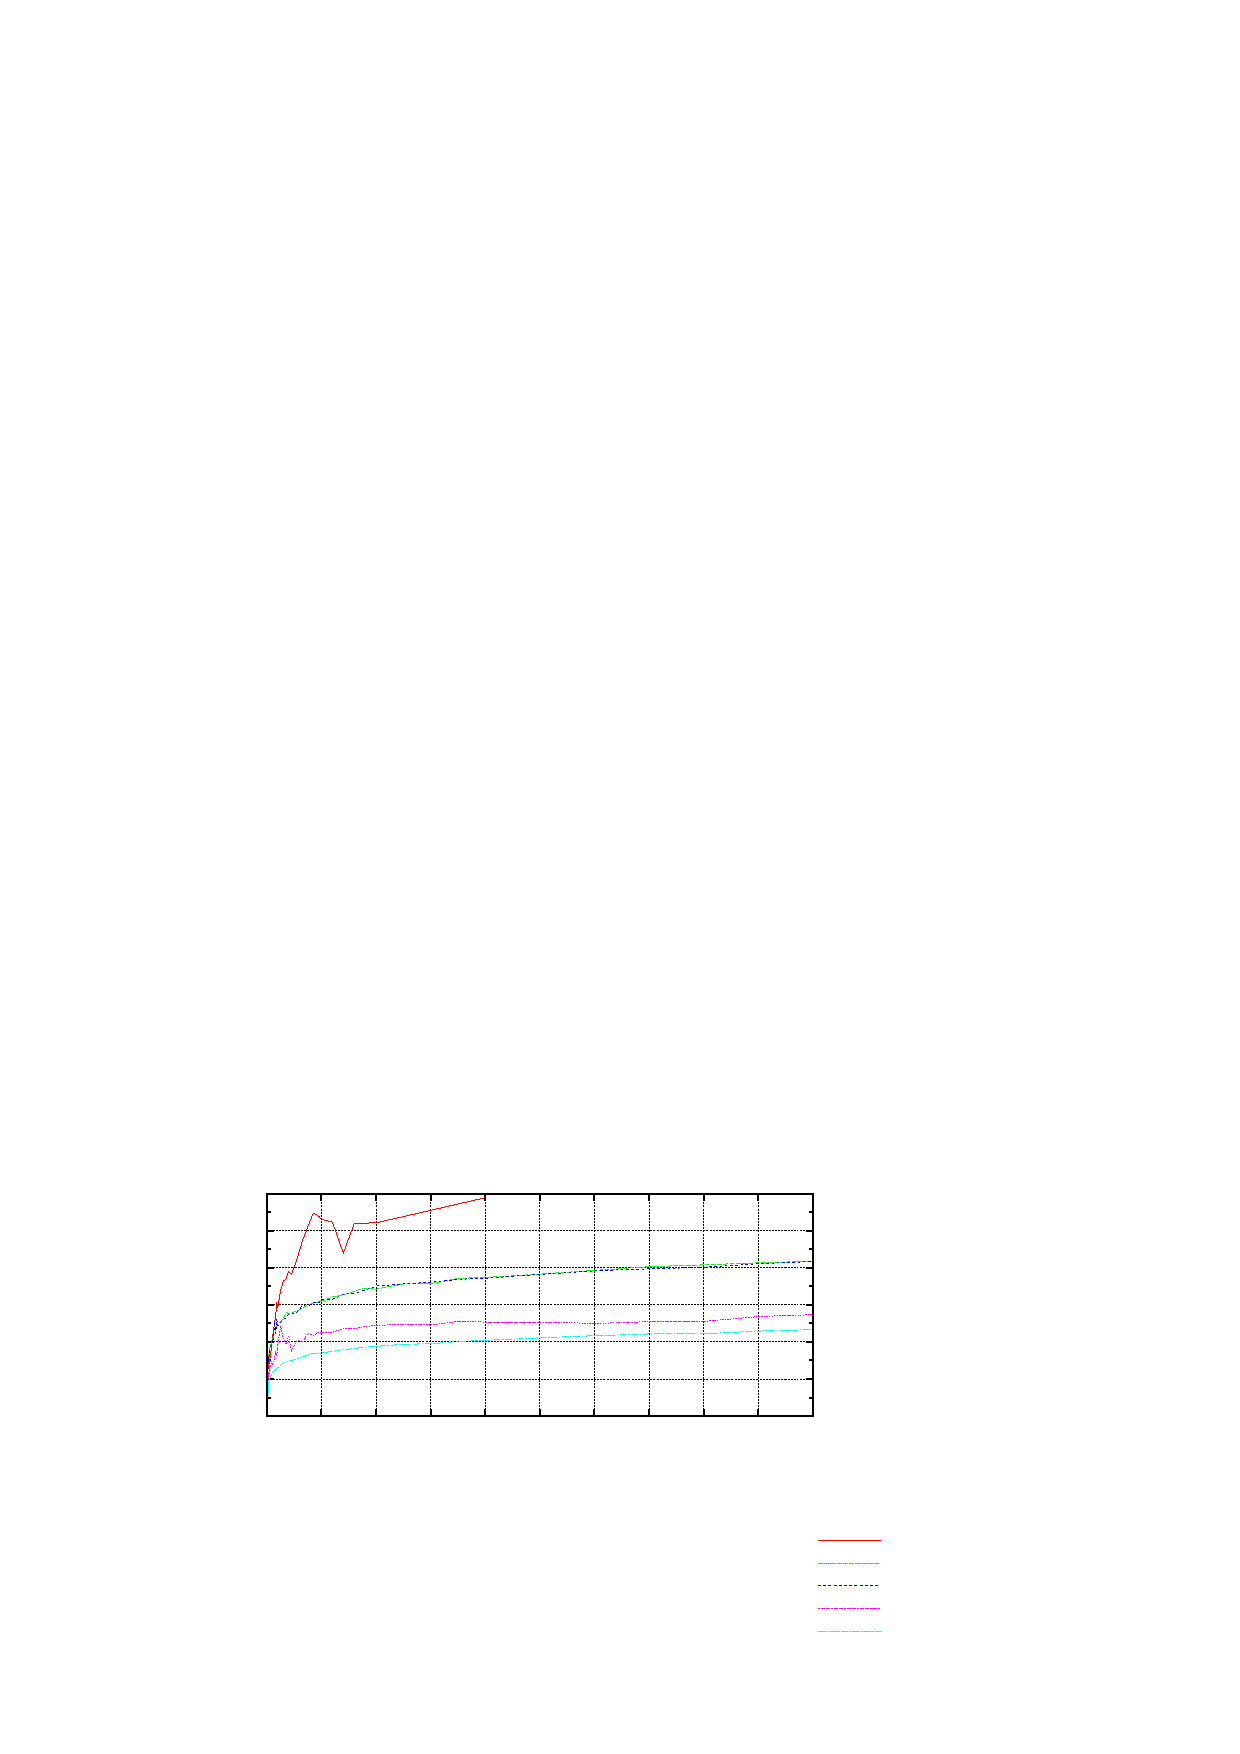
\includegraphics{ej4_nodos_connected_regular}}%
    \gplfronttext
  \end{picture}%
\endgroup
}
    \caption{Complejidad temporal para Grafos Conexos Regulares}
\end{figure}

\begin{figure}[H]
    \centering
    \fontsize{7}{10}\selectfont
    \resizebox{0.80\textwidth}{!}{% GNUPLOT: LaTeX picture with Postscript
\begingroup
  \makeatletter
  \providecommand\color[2][]{%
    \GenericError{(gnuplot) \space\space\space\@spaces}{%
      Package color not loaded in conjunction with
      terminal option `colourtext'%
    }{See the gnuplot documentation for explanation.%
    }{Either use 'blacktext' in gnuplot or load the package
      color.sty in LaTeX.}%
    \renewcommand\color[2][]{}%
  }%
  \providecommand\includegraphics[2][]{%
    \GenericError{(gnuplot) \space\space\space\@spaces}{%
      Package graphicx or graphics not loaded%
    }{See the gnuplot documentation for explanation.%
    }{The gnuplot epslatex terminal needs graphicx.sty or graphics.sty.}%
    \renewcommand\includegraphics[2][]{}%
  }%
  \providecommand\rotatebox[2]{#2}%
  \@ifundefined{ifGPcolor}{%
    \newif\ifGPcolor
    \GPcolortrue
  }{}%
  \@ifundefined{ifGPblacktext}{%
    \newif\ifGPblacktext
    \GPblacktexttrue
  }{}%
  % define a \g@addto@macro without @ in the name:
  \let\gplgaddtomacro\g@addto@macro
  % define empty templates for all commands taking text:
  \gdef\gplbacktext{}%
  \gdef\gplfronttext{}%
  \makeatother
  \ifGPblacktext
    % no textcolor at all
    \def\colorrgb#1{}%
    \def\colorgray#1{}%
  \else
    % gray or color?
    \ifGPcolor
      \def\colorrgb#1{\color[rgb]{#1}}%
      \def\colorgray#1{\color[gray]{#1}}%
      \expandafter\def\csname LTw\endcsname{\color{white}}%
      \expandafter\def\csname LTb\endcsname{\color{black}}%
      \expandafter\def\csname LTa\endcsname{\color{black}}%
      \expandafter\def\csname LT0\endcsname{\color[rgb]{1,0,0}}%
      \expandafter\def\csname LT1\endcsname{\color[rgb]{0,1,0}}%
      \expandafter\def\csname LT2\endcsname{\color[rgb]{0,0,1}}%
      \expandafter\def\csname LT3\endcsname{\color[rgb]{1,0,1}}%
      \expandafter\def\csname LT4\endcsname{\color[rgb]{0,1,1}}%
      \expandafter\def\csname LT5\endcsname{\color[rgb]{1,1,0}}%
      \expandafter\def\csname LT6\endcsname{\color[rgb]{0,0,0}}%
      \expandafter\def\csname LT7\endcsname{\color[rgb]{1,0.3,0}}%
      \expandafter\def\csname LT8\endcsname{\color[rgb]{0.5,0.5,0.5}}%
    \else
      % gray
      \def\colorrgb#1{\color{black}}%
      \def\colorgray#1{\color[gray]{#1}}%
      \expandafter\def\csname LTw\endcsname{\color{white}}%
      \expandafter\def\csname LTb\endcsname{\color{black}}%
      \expandafter\def\csname LTa\endcsname{\color{black}}%
      \expandafter\def\csname LT0\endcsname{\color{black}}%
      \expandafter\def\csname LT1\endcsname{\color{black}}%
      \expandafter\def\csname LT2\endcsname{\color{black}}%
      \expandafter\def\csname LT3\endcsname{\color{black}}%
      \expandafter\def\csname LT4\endcsname{\color{black}}%
      \expandafter\def\csname LT5\endcsname{\color{black}}%
      \expandafter\def\csname LT6\endcsname{\color{black}}%
      \expandafter\def\csname LT7\endcsname{\color{black}}%
      \expandafter\def\csname LT8\endcsname{\color{black}}%
    \fi
  \fi
  \setlength{\unitlength}{0.0500bp}%
  \begin{picture}(7200.00,5040.00)%
    \gplgaddtomacro\gplbacktext{%
      \csname LTb\endcsname%
      \put(1430,2244){\makebox(0,0)[r]{\strut{} 0}}%
      \csname LTb\endcsname%
      \put(1430,2600){\makebox(0,0)[r]{\strut{} 10000}}%
      \csname LTb\endcsname%
      \put(1430,2956){\makebox(0,0)[r]{\strut{} 20000}}%
      \csname LTb\endcsname%
      \put(1430,3312){\makebox(0,0)[r]{\strut{} 30000}}%
      \csname LTb\endcsname%
      \put(1430,3667){\makebox(0,0)[r]{\strut{} 40000}}%
      \csname LTb\endcsname%
      \put(1430,4023){\makebox(0,0)[r]{\strut{} 50000}}%
      \csname LTb\endcsname%
      \put(1430,4379){\makebox(0,0)[r]{\strut{} 60000}}%
      \csname LTb\endcsname%
      \put(1562,2024){\makebox(0,0){\strut{} 0}}%
      \csname LTb\endcsname%
      \put(2086,2024){\makebox(0,0){\strut{} 500}}%
      \csname LTb\endcsname%
      \put(2610,2024){\makebox(0,0){\strut{} 1000}}%
      \csname LTb\endcsname%
      \put(3134,2024){\makebox(0,0){\strut{} 1500}}%
      \csname LTb\endcsname%
      \put(3658,2024){\makebox(0,0){\strut{} 2000}}%
      \csname LTb\endcsname%
      \put(4183,2024){\makebox(0,0){\strut{} 2500}}%
      \csname LTb\endcsname%
      \put(4707,2024){\makebox(0,0){\strut{} 3000}}%
      \csname LTb\endcsname%
      \put(5231,2024){\makebox(0,0){\strut{} 3500}}%
      \csname LTb\endcsname%
      \put(5755,2024){\makebox(0,0){\strut{} 4000}}%
      \csname LTb\endcsname%
      \put(6279,2024){\makebox(0,0){\strut{} 4500}}%
      \csname LTb\endcsname%
      \put(6803,2024){\makebox(0,0){\strut{} 5000}}%
      \put(176,3311){\rotatebox{-270}{\makebox(0,0){\strut{}Frontera}}}%
      \put(396,3311){\rotatebox{-270}{\makebox(0,0){\strut{}(Escala Lineal)}}}%
      \put(4182,1694){\makebox(0,0){\strut{}Cantidad de Nodos}}%
      \put(4182,1474){\makebox(0,0){\strut{}(Escala Lineal)}}%
      \put(4182,4709){\makebox(0,0){\strut{}Frontera obtenida segun cantidad de nodos}}%
    }%
    \gplgaddtomacro\gplfronttext{%
      \csname LTb\endcsname%
      \put(6725,1053){\makebox(0,0)[r]{\strut{}Algoritmo Exacto (Regular)}}%
      \csname LTb\endcsname%
      \put(6725,833){\makebox(0,0)[r]{\strut{}Tabu(n,n,n/2) (golosa,sin aspiracion,regular)}}%
      \csname LTb\endcsname%
      \put(6725,613){\makebox(0,0)[r]{\strut{}Tabu(n,n,n/2,regular)}}%
      \csname LTb\endcsname%
      \put(6725,393){\makebox(0,0)[r]{\strut{}BL (mejor vecino,intercambio,regular)}}%
      \csname LTb\endcsname%
      \put(6725,173){\makebox(0,0)[r]{\strut{}Golosa (regular)}}%
    }%
    \gplbacktext
    \put(0,0){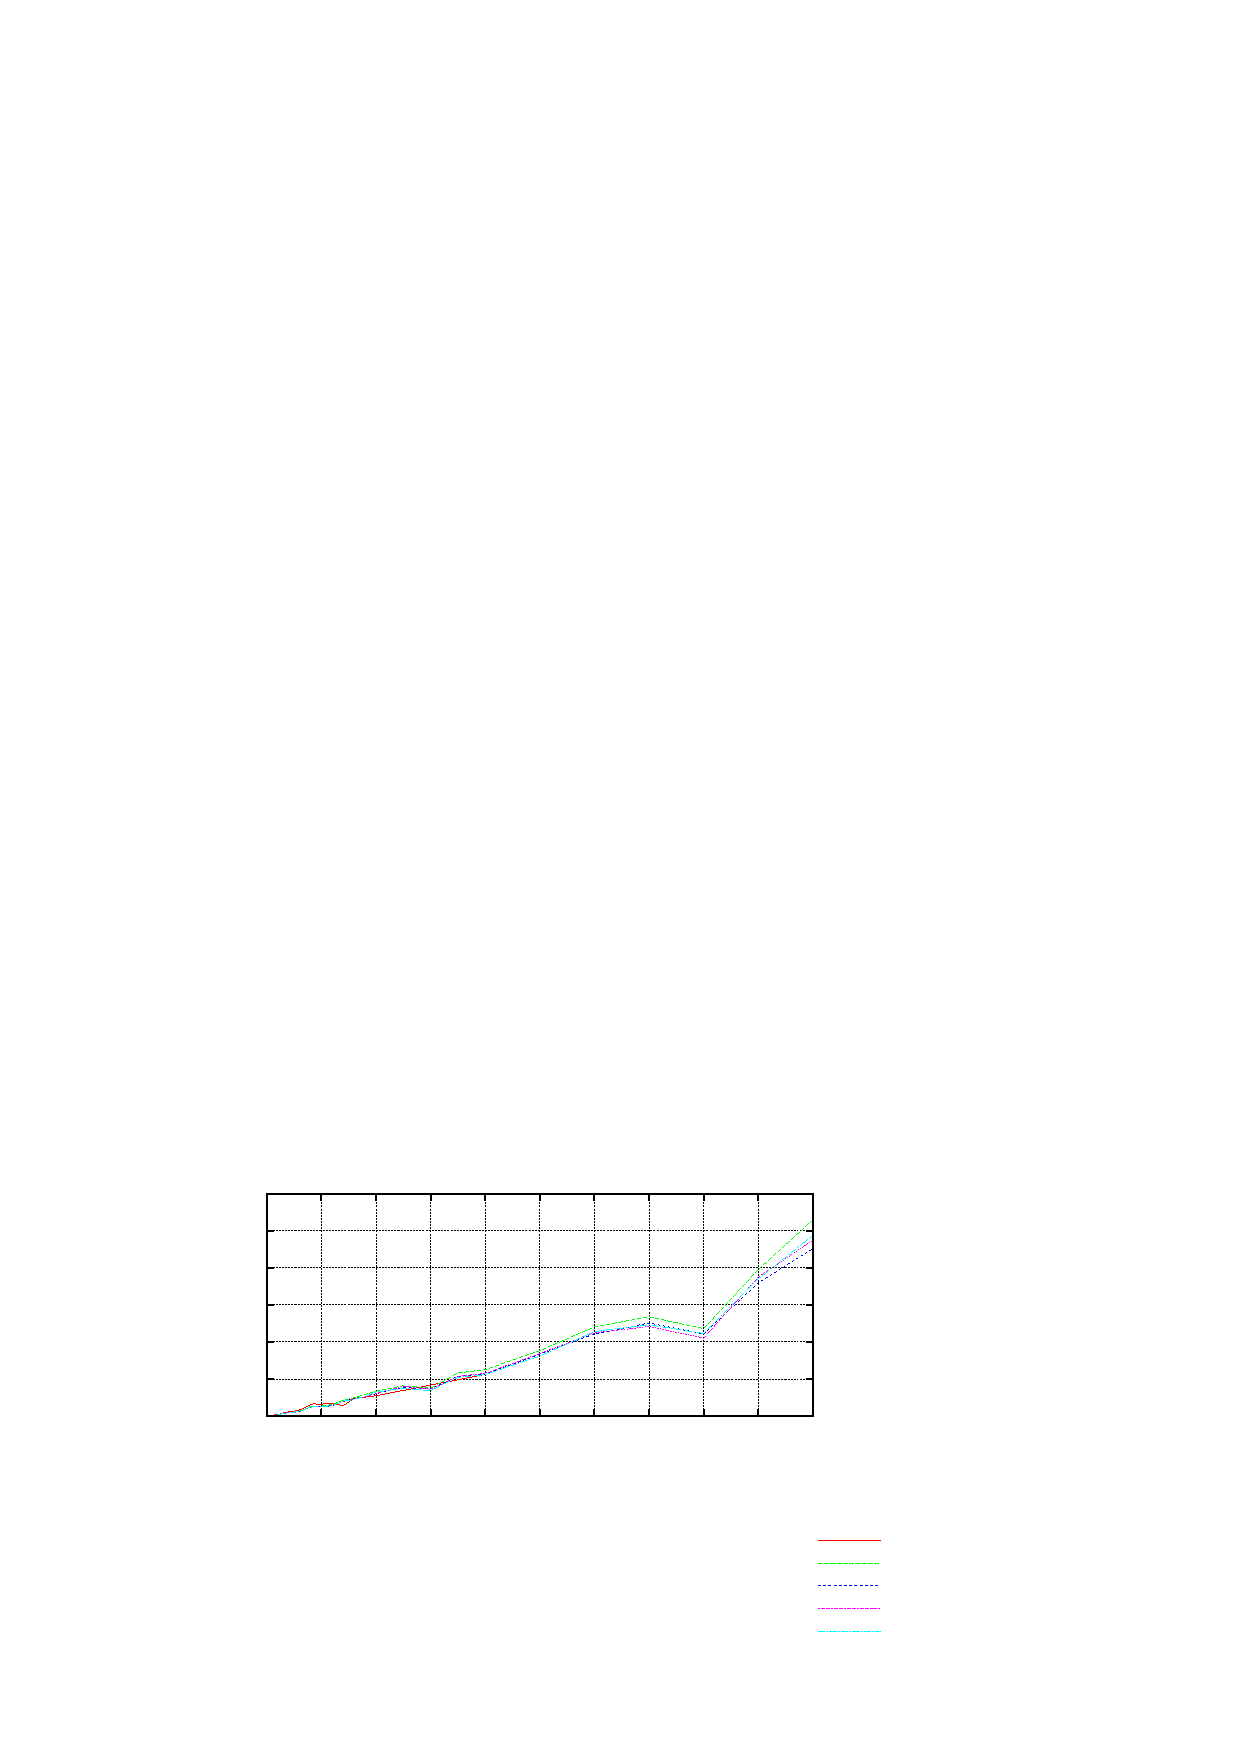
\includegraphics{ej4_frontera_connected_regular}}%
    \gplfronttext
  \end{picture}%
\endgroup
}
    \caption{Frontera para Grafos Conexos Regulares}
\end{figure}


\bigskip

\par Para esta familia de grafos m\'as densos, vemos que los
    resultados obtenidos se mantienen, si bien ya las heur\'isticas
    comienzan a estar cada vez m\'as cerca, tanto en resultado provisto
    como en sus tiempo s de ejecuci\'on. A\'un as\'i, la heur\'istica 
    golosa siguie teniendo la ventaja respecto de las dem\'as y mientras
    que el resultado provisto por todas las heur\'isticas son similares
    (y vale la pena mencionar, hasta los grafos de 200 nodos se
    puede observar como todas las variantes de las heur\'isticas
    que est\'an siendo evaluadas dan resultados sumamente aceptables).

\subsubsection{Grafos muy densos}
%Connected Dense
\begin{figure}[H]
    \centering
    \fontsize{7}{10}\selectfont
    \resizebox{0.80\textwidth}{!}{% GNUPLOT: LaTeX picture with Postscript
\begingroup
  \makeatletter
  \providecommand\color[2][]{%
    \GenericError{(gnuplot) \space\space\space\@spaces}{%
      Package color not loaded in conjunction with
      terminal option `colourtext'%
    }{See the gnuplot documentation for explanation.%
    }{Either use 'blacktext' in gnuplot or load the package
      color.sty in LaTeX.}%
    \renewcommand\color[2][]{}%
  }%
  \providecommand\includegraphics[2][]{%
    \GenericError{(gnuplot) \space\space\space\@spaces}{%
      Package graphicx or graphics not loaded%
    }{See the gnuplot documentation for explanation.%
    }{The gnuplot epslatex terminal needs graphicx.sty or graphics.sty.}%
    \renewcommand\includegraphics[2][]{}%
  }%
  \providecommand\rotatebox[2]{#2}%
  \@ifundefined{ifGPcolor}{%
    \newif\ifGPcolor
    \GPcolortrue
  }{}%
  \@ifundefined{ifGPblacktext}{%
    \newif\ifGPblacktext
    \GPblacktexttrue
  }{}%
  % define a \g@addto@macro without @ in the name:
  \let\gplgaddtomacro\g@addto@macro
  % define empty templates for all commands taking text:
  \gdef\gplbacktext{}%
  \gdef\gplfronttext{}%
  \makeatother
  \ifGPblacktext
    % no textcolor at all
    \def\colorrgb#1{}%
    \def\colorgray#1{}%
  \else
    % gray or color?
    \ifGPcolor
      \def\colorrgb#1{\color[rgb]{#1}}%
      \def\colorgray#1{\color[gray]{#1}}%
      \expandafter\def\csname LTw\endcsname{\color{white}}%
      \expandafter\def\csname LTb\endcsname{\color{black}}%
      \expandafter\def\csname LTa\endcsname{\color{black}}%
      \expandafter\def\csname LT0\endcsname{\color[rgb]{1,0,0}}%
      \expandafter\def\csname LT1\endcsname{\color[rgb]{0,1,0}}%
      \expandafter\def\csname LT2\endcsname{\color[rgb]{0,0,1}}%
      \expandafter\def\csname LT3\endcsname{\color[rgb]{1,0,1}}%
      \expandafter\def\csname LT4\endcsname{\color[rgb]{0,1,1}}%
      \expandafter\def\csname LT5\endcsname{\color[rgb]{1,1,0}}%
      \expandafter\def\csname LT6\endcsname{\color[rgb]{0,0,0}}%
      \expandafter\def\csname LT7\endcsname{\color[rgb]{1,0.3,0}}%
      \expandafter\def\csname LT8\endcsname{\color[rgb]{0.5,0.5,0.5}}%
    \else
      % gray
      \def\colorrgb#1{\color{black}}%
      \def\colorgray#1{\color[gray]{#1}}%
      \expandafter\def\csname LTw\endcsname{\color{white}}%
      \expandafter\def\csname LTb\endcsname{\color{black}}%
      \expandafter\def\csname LTa\endcsname{\color{black}}%
      \expandafter\def\csname LT0\endcsname{\color{black}}%
      \expandafter\def\csname LT1\endcsname{\color{black}}%
      \expandafter\def\csname LT2\endcsname{\color{black}}%
      \expandafter\def\csname LT3\endcsname{\color{black}}%
      \expandafter\def\csname LT4\endcsname{\color{black}}%
      \expandafter\def\csname LT5\endcsname{\color{black}}%
      \expandafter\def\csname LT6\endcsname{\color{black}}%
      \expandafter\def\csname LT7\endcsname{\color{black}}%
      \expandafter\def\csname LT8\endcsname{\color{black}}%
    \fi
  \fi
  \setlength{\unitlength}{0.0500bp}%
  \begin{picture}(7200.00,5040.00)%
    \gplgaddtomacro\gplbacktext{%
      \csname LTb\endcsname%
      \put(1430,2244){\makebox(0,0)[r]{\strut{} 0.01}}%
      \csname LTb\endcsname%
      \put(1430,2600){\makebox(0,0)[r]{\strut{} 1}}%
      \csname LTb\endcsname%
      \put(1430,2956){\makebox(0,0)[r]{\strut{} 100}}%
      \csname LTb\endcsname%
      \put(1430,3312){\makebox(0,0)[r]{\strut{} 10000}}%
      \csname LTb\endcsname%
      \put(1430,3667){\makebox(0,0)[r]{\strut{} 1e+06}}%
      \csname LTb\endcsname%
      \put(1430,4023){\makebox(0,0)[r]{\strut{} 1e+08}}%
      \csname LTb\endcsname%
      \put(1430,4379){\makebox(0,0)[r]{\strut{} 1e+10}}%
      \csname LTb\endcsname%
      \put(1562,2024){\makebox(0,0){\strut{} 0}}%
      \csname LTb\endcsname%
      \put(2086,2024){\makebox(0,0){\strut{} 500}}%
      \csname LTb\endcsname%
      \put(2610,2024){\makebox(0,0){\strut{} 1000}}%
      \csname LTb\endcsname%
      \put(3134,2024){\makebox(0,0){\strut{} 1500}}%
      \csname LTb\endcsname%
      \put(3658,2024){\makebox(0,0){\strut{} 2000}}%
      \csname LTb\endcsname%
      \put(4183,2024){\makebox(0,0){\strut{} 2500}}%
      \csname LTb\endcsname%
      \put(4707,2024){\makebox(0,0){\strut{} 3000}}%
      \csname LTb\endcsname%
      \put(5231,2024){\makebox(0,0){\strut{} 3500}}%
      \csname LTb\endcsname%
      \put(5755,2024){\makebox(0,0){\strut{} 4000}}%
      \csname LTb\endcsname%
      \put(6279,2024){\makebox(0,0){\strut{} 4500}}%
      \csname LTb\endcsname%
      \put(6803,2024){\makebox(0,0){\strut{} 5000}}%
      \put(176,3311){\rotatebox{-270}{\makebox(0,0){\strut{}Tiempo (microsegundos)}}}%
      \put(396,3311){\rotatebox{-270}{\makebox(0,0){\strut{}(Escala Logaritmica)}}}%
      \put(4182,1694){\makebox(0,0){\strut{}Cantidad de Nodos}}%
      \put(4182,1474){\makebox(0,0){\strut{}(Escala Lineal)}}%
      \put(4182,4709){\makebox(0,0){\strut{}Tiempo de ejecucion conforme aumenta la cantidad de nodos}}%
    }%
    \gplgaddtomacro\gplfronttext{%
      \csname LTb\endcsname%
      \put(6593,1053){\makebox(0,0)[r]{\strut{}Algoritmo Exacto (Denso)}}%
      \csname LTb\endcsname%
      \put(6593,833){\makebox(0,0)[r]{\strut{}Tabu(n,n,n/2) (golosa,sin aspiracion,denso)}}%
      \csname LTb\endcsname%
      \put(6593,613){\makebox(0,0)[r]{\strut{}Tabu(n,n,n/2,denso)}}%
      \csname LTb\endcsname%
      \put(6593,393){\makebox(0,0)[r]{\strut{}BL (mejor vecino,intercambio,denso)}}%
      \csname LTb\endcsname%
      \put(6593,173){\makebox(0,0)[r]{\strut{}Golosa (denso)}}%
    }%
    \gplbacktext
    \put(0,0){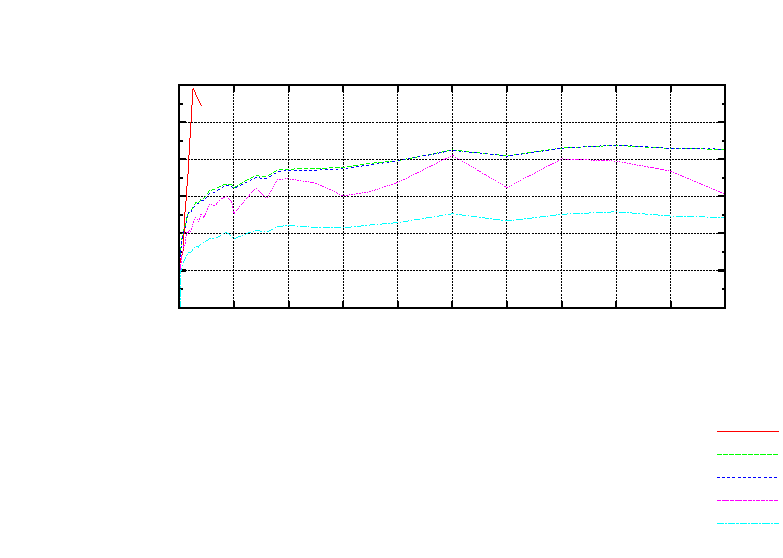
\includegraphics{ej4_nodos_connected_dense}}%
    \gplfronttext
  \end{picture}%
\endgroup
}
    \caption{Complejidad temporal para Grafos Conexos Densos}
\end{figure}

\begin{figure}[H]
    \centering
    \fontsize{7}{10}\selectfont
    \resizebox{0.80\textwidth}{!}{% GNUPLOT: LaTeX picture with Postscript
\begingroup
  \makeatletter
  \providecommand\color[2][]{%
    \GenericError{(gnuplot) \space\space\space\@spaces}{%
      Package color not loaded in conjunction with
      terminal option `colourtext'%
    }{See the gnuplot documentation for explanation.%
    }{Either use 'blacktext' in gnuplot or load the package
      color.sty in LaTeX.}%
    \renewcommand\color[2][]{}%
  }%
  \providecommand\includegraphics[2][]{%
    \GenericError{(gnuplot) \space\space\space\@spaces}{%
      Package graphicx or graphics not loaded%
    }{See the gnuplot documentation for explanation.%
    }{The gnuplot epslatex terminal needs graphicx.sty or graphics.sty.}%
    \renewcommand\includegraphics[2][]{}%
  }%
  \providecommand\rotatebox[2]{#2}%
  \@ifundefined{ifGPcolor}{%
    \newif\ifGPcolor
    \GPcolortrue
  }{}%
  \@ifundefined{ifGPblacktext}{%
    \newif\ifGPblacktext
    \GPblacktexttrue
  }{}%
  % define a \g@addto@macro without @ in the name:
  \let\gplgaddtomacro\g@addto@macro
  % define empty templates for all commands taking text:
  \gdef\gplbacktext{}%
  \gdef\gplfronttext{}%
  \makeatother
  \ifGPblacktext
    % no textcolor at all
    \def\colorrgb#1{}%
    \def\colorgray#1{}%
  \else
    % gray or color?
    \ifGPcolor
      \def\colorrgb#1{\color[rgb]{#1}}%
      \def\colorgray#1{\color[gray]{#1}}%
      \expandafter\def\csname LTw\endcsname{\color{white}}%
      \expandafter\def\csname LTb\endcsname{\color{black}}%
      \expandafter\def\csname LTa\endcsname{\color{black}}%
      \expandafter\def\csname LT0\endcsname{\color[rgb]{1,0,0}}%
      \expandafter\def\csname LT1\endcsname{\color[rgb]{0,1,0}}%
      \expandafter\def\csname LT2\endcsname{\color[rgb]{0,0,1}}%
      \expandafter\def\csname LT3\endcsname{\color[rgb]{1,0,1}}%
      \expandafter\def\csname LT4\endcsname{\color[rgb]{0,1,1}}%
      \expandafter\def\csname LT5\endcsname{\color[rgb]{1,1,0}}%
      \expandafter\def\csname LT6\endcsname{\color[rgb]{0,0,0}}%
      \expandafter\def\csname LT7\endcsname{\color[rgb]{1,0.3,0}}%
      \expandafter\def\csname LT8\endcsname{\color[rgb]{0.5,0.5,0.5}}%
    \else
      % gray
      \def\colorrgb#1{\color{black}}%
      \def\colorgray#1{\color[gray]{#1}}%
      \expandafter\def\csname LTw\endcsname{\color{white}}%
      \expandafter\def\csname LTb\endcsname{\color{black}}%
      \expandafter\def\csname LTa\endcsname{\color{black}}%
      \expandafter\def\csname LT0\endcsname{\color{black}}%
      \expandafter\def\csname LT1\endcsname{\color{black}}%
      \expandafter\def\csname LT2\endcsname{\color{black}}%
      \expandafter\def\csname LT3\endcsname{\color{black}}%
      \expandafter\def\csname LT4\endcsname{\color{black}}%
      \expandafter\def\csname LT5\endcsname{\color{black}}%
      \expandafter\def\csname LT6\endcsname{\color{black}}%
      \expandafter\def\csname LT7\endcsname{\color{black}}%
      \expandafter\def\csname LT8\endcsname{\color{black}}%
    \fi
  \fi
  \setlength{\unitlength}{0.0500bp}%
  \begin{picture}(7200.00,5040.00)%
    \gplgaddtomacro\gplbacktext{%
      \csname LTb\endcsname%
      \put(1562,2244){\makebox(0,0)[r]{\strut{} 0}}%
      \csname LTb\endcsname%
      \put(1562,2481){\makebox(0,0)[r]{\strut{} 50000}}%
      \csname LTb\endcsname%
      \put(1562,2718){\makebox(0,0)[r]{\strut{} 100000}}%
      \csname LTb\endcsname%
      \put(1562,2956){\makebox(0,0)[r]{\strut{} 150000}}%
      \csname LTb\endcsname%
      \put(1562,3193){\makebox(0,0)[r]{\strut{} 200000}}%
      \csname LTb\endcsname%
      \put(1562,3430){\makebox(0,0)[r]{\strut{} 250000}}%
      \csname LTb\endcsname%
      \put(1562,3667){\makebox(0,0)[r]{\strut{} 300000}}%
      \csname LTb\endcsname%
      \put(1562,3905){\makebox(0,0)[r]{\strut{} 350000}}%
      \csname LTb\endcsname%
      \put(1562,4142){\makebox(0,0)[r]{\strut{} 400000}}%
      \csname LTb\endcsname%
      \put(1562,4379){\makebox(0,0)[r]{\strut{} 450000}}%
      \csname LTb\endcsname%
      \put(1694,2024){\makebox(0,0){\strut{} 1500}}%
      \csname LTb\endcsname%
      \put(2424,2024){\makebox(0,0){\strut{} 2000}}%
      \csname LTb\endcsname%
      \put(3154,2024){\makebox(0,0){\strut{} 2500}}%
      \csname LTb\endcsname%
      \put(3884,2024){\makebox(0,0){\strut{} 3000}}%
      \csname LTb\endcsname%
      \put(4613,2024){\makebox(0,0){\strut{} 3500}}%
      \csname LTb\endcsname%
      \put(5343,2024){\makebox(0,0){\strut{} 4000}}%
      \csname LTb\endcsname%
      \put(6073,2024){\makebox(0,0){\strut{} 4500}}%
      \csname LTb\endcsname%
      \put(6803,2024){\makebox(0,0){\strut{} 5000}}%
      \put(176,3311){\rotatebox{-270}{\makebox(0,0){\strut{}Frontera}}}%
      \put(396,3311){\rotatebox{-270}{\makebox(0,0){\strut{}(Escala Lineal)}}}%
      \put(4248,1694){\makebox(0,0){\strut{}Cantidad de Nodos}}%
      \put(4248,1474){\makebox(0,0){\strut{}(Escala Lineal)}}%
      \put(4248,4709){\makebox(0,0){\strut{}Frontera obtenida segun cantidad de nodos}}%
    }%
    \gplgaddtomacro\gplfronttext{%
      \csname LTb\endcsname%
      \put(6659,1053){\makebox(0,0)[r]{\strut{}Algoritmo Exacto (Denso)}}%
      \csname LTb\endcsname%
      \put(6659,833){\makebox(0,0)[r]{\strut{}Tabu(n,n,n/2) (golosa,sin aspiracion,denso)}}%
      \csname LTb\endcsname%
      \put(6659,613){\makebox(0,0)[r]{\strut{}Tabu(n,n,n/2,denso)}}%
      \csname LTb\endcsname%
      \put(6659,393){\makebox(0,0)[r]{\strut{}BL (mejor vecino,intercambio,denso)}}%
      \csname LTb\endcsname%
      \put(6659,173){\makebox(0,0)[r]{\strut{}Golosa (denso)}}%
    }%
    \gplbacktext
    \put(0,0){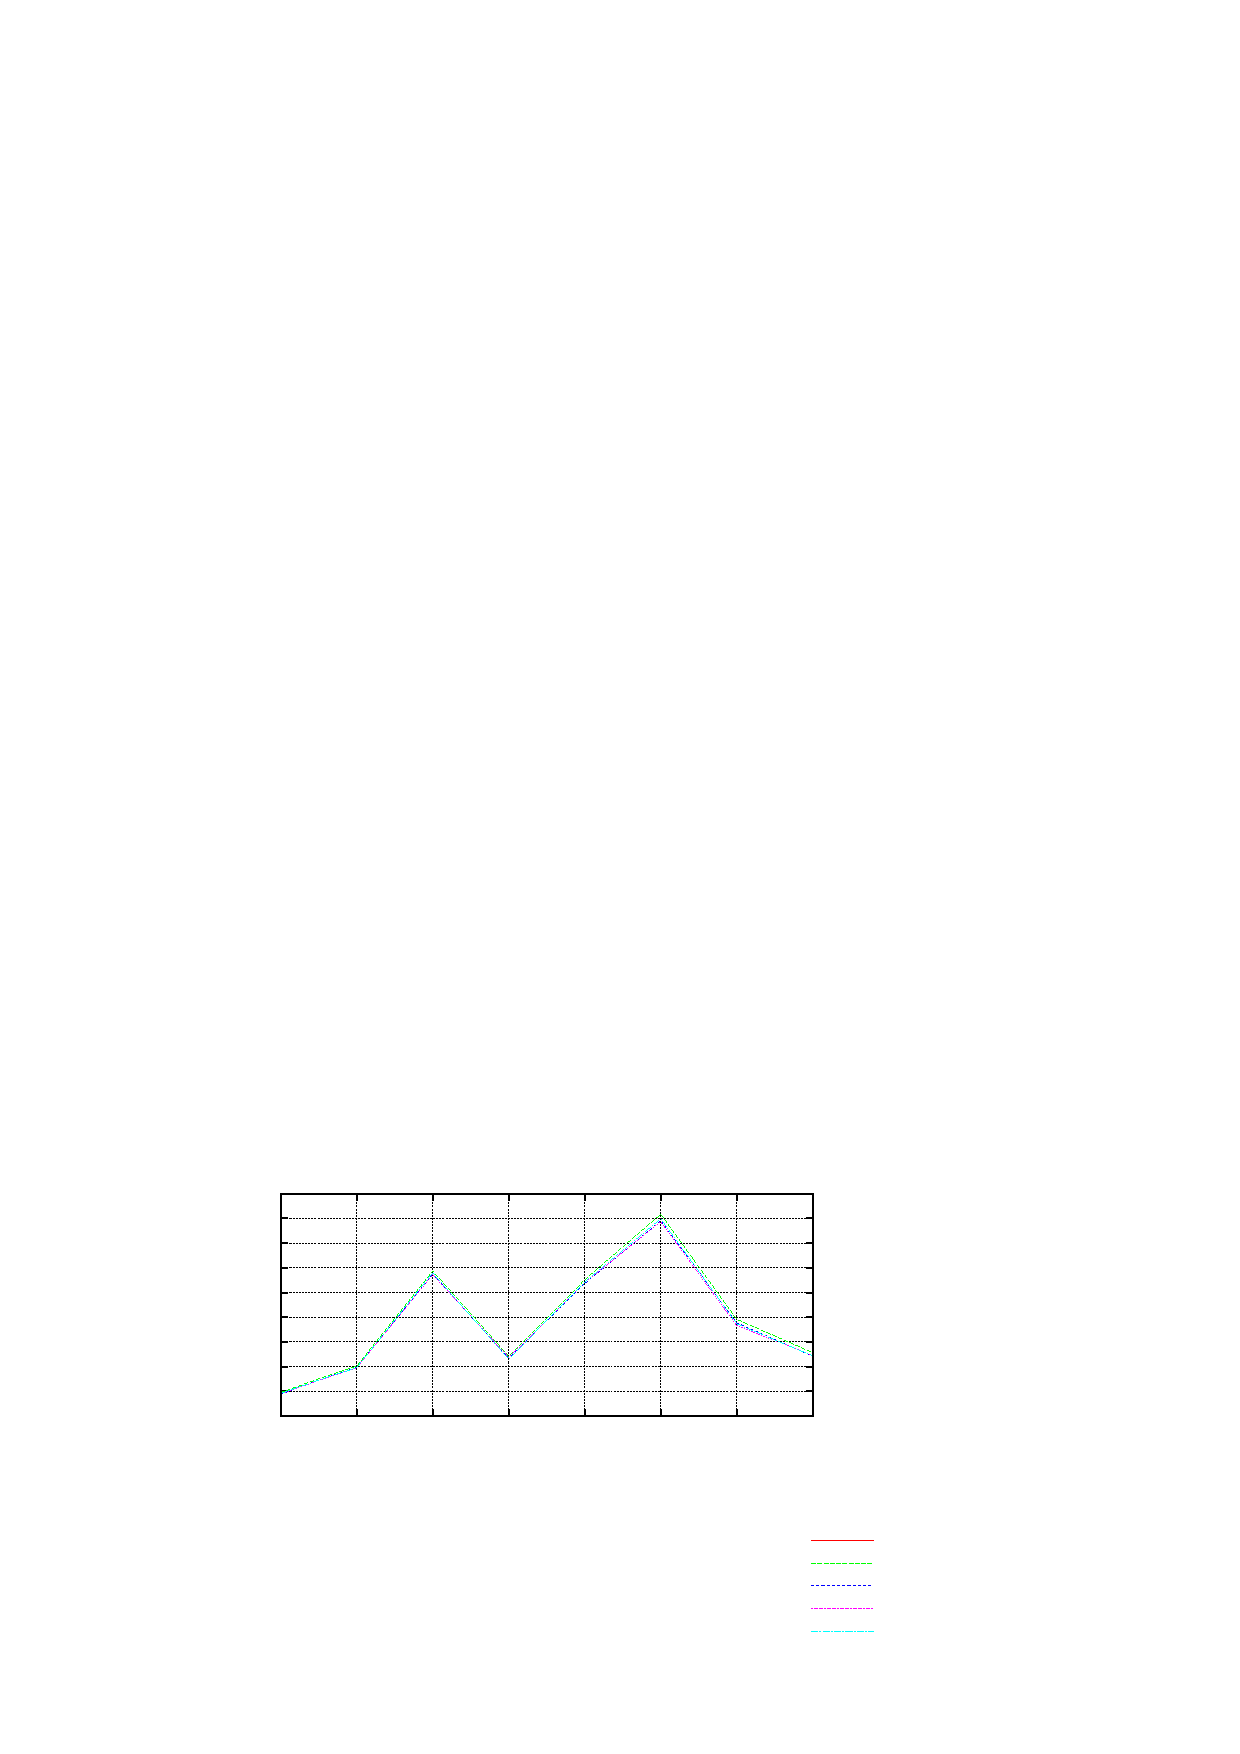
\includegraphics{ej4_frontera_connected_dense}}%
    \gplfronttext
  \end{picture}%
\endgroup
}
    \caption{Frontera para Grafos Conexos Densos}
\end{figure}

\bigskip

\par Por \'ultimo, observamos como los resultados, si bien se mantienen,
    siguen acerc\'andose. Al menos hasta los 5000 nodos, la soluci\'on
    golosa se ha eregido como la elegida a la hora de resolver dichos
    problemas si no se tiene informaci\'on sobre la estructura de los
    grafos de entrada.

\subsection{Conclusiones}
\par Para finalizar este trabajo, vale la pena mencionar que quedaron
    muchas variantes de las heur\'isticas (especialmente de la b\'usqueda
    tab\'u) y de muchas otras familias de grafo para las cuales los
    resultados, seguramente, hubieran sido diferentes.

\par Como conclusiones, debemos afirmar que este \'ultimo an\'alisis
    global realizado se hizo sin tener informaci\'on de los grafos
    que modelan los problemas que se desean resolver. Dicha informaci\'on
    puede ser (de hecho, es lo principal) muy importante, sino cr\'itico,
    a la hora de desarrollar una heur\'istica (cosa que es necesaria
    si llegar a una soluci\'on \'optima para el problema es muy caro
    computacionalmente).

\par Al no tener dicha informaci\'on, se decidi\'o hacer unas heur\'isticas
    un tanto g\'enericas para un problema particular, y los resultados
    obteniods de la experimentaci\'on no son, ni est\'an cerca de serlo,
    concluyentes sobre que heur\'istica es ``mejor'' para resolver el
    problema de \emph{CMF}\footnote{En particular, como no se saben
    cuan buena alcanza que sea la soluci\'on obtenida, ni el tiempo
    m\'aximo que se est\'a dispuesto a esperar por ella, la definici\'on
    de ``mejor heur\'istica'' carace, en parte, de sentido.}.
